\documentclass[11pt, a4paper]{article}

\usepackage[utf8]{inputenc}
\usepackage[T1]{fontenc}
\usepackage[provide=*]{babel}
\babelprovide[import, main]{spanish}
\usepackage{geometry}
\geometry{left=2.5cm, right=2.5cm, top=2.5cm, bottom=2.5cm}
\usepackage{graphicx}
\usepackage{float}
\usepackage{amssymb}
\usepackage{booktabs}
\usepackage{array}
\usepackage{longtable}
\usepackage{enumitem}
\usepackage{xcolor}
\usepackage{fancyhdr}
\usepackage{listings}
\usepackage{tikz}
\usetikzlibrary{positioning, arrows.meta, shapes.geometric, fit, backgrounds}
\usepackage{hyperref}

\definecolor{azulUH}{RGB}{0,51,102}
\definecolor{grisUH}{RGB}{90,90,90}
\definecolor{fondocod}{RGB}{245,246,248}
\definecolor{sqlcol}{RGB}{68,121,161}
\definecolor{mongocol}{RGB}{71,162,72}
\definecolor{neocol}{RGB}{0,140,193}

\hypersetup{
    colorlinks=true,
    linkcolor=azulUH,
    urlcolor=azulUH,
    citecolor=azulUH,
    pdftitle={Informe Técnico - Proyecto AquaLife},
    pdfauthor={Alejandro de la Torre (amnesiac-ds), Fabián Cabrera Delgado (fcd06), Darío Quintana Roque (darioqr)}
}

\lstset{
    basicstyle=\ttfamily\footnotesize,
    backgroundcolor=\color{fondocod},
    frame=single,
    rulecolor=\color{grisUH!40},
    breaklines=true,
    columns=fullflexible,
    keepspaces=true,
    xleftmargin=0.5em,
    xrightmargin=0.5em,
    aboveskip=0.8em,
    belowskip=0.8em
}

\setlength{\parskip}{0.45em}
\setlength{\emergencystretch}{3em}
\tolerance=1500
\setlength{\parindent}{0pt}
\renewcommand{\arraystretch}{1.25}

\pagestyle{fancy}
\fancyhf{}
\fancyhead[L]{\small\color{grisUH} Informe Técnico -- AquaLife}
\fancyhead[R]{\small\color{grisUH} Bases de Datos, Curso 2026}
\fancyfoot[C]{\small\thepage}
\renewcommand{\headrulewidth}{0.3pt}

\newcommand{\sql}{\texttt}
\newcommand{\nota}[1]{\par\smallskip\noindent\textit{\color{grisUH}#1}\par\smallskip}

\title{\textbf{Informe Técnico}\\[0.4em]\Large Proyecto AquaLife: persistencia políglota con\\MySQL, MongoDB y Neo4j}
\author{Alejandro de la Torre (amnesiac-ds) \and Fabián Cabrera Delgado (fcd06) \and Darío Quintana Roque (darioqr)}
\date{\today}

\begin{document}

\maketitle
\thispagestyle{fancy}

\begin{abstract}
\noindent
AquaLife es un sistema de información para una comunidad acuática que combina tres paradigmas de bases de datos: relacional (MySQL), documental (MongoDB) y de grafos (Neo4j). Este informe documenta la arquitectura global del proyecto, el modelo relacional y sus consultas analíticas, y justifica la elección de cada modelo NoSQL: MongoDB para la documentación jerárquica de especies y Neo4j para las conversaciones en hilos de comentarios, que se contrasta con una implementación relacional equivalente. Se incluye una comparación global de los tres modelos y un apartado de limitaciones y mejoras detectadas durante la revisión del repositorio.
\end{abstract}

\tableofcontents
\newpage

%=====================================================================
\section{Introducción y alcance}
%=====================================================================

\subsection{Descripción del proyecto}
AquaLife es el proyecto final de la asignatura de Bases de Datos. El dominio es una comunidad de acuarismo: usuarios que publican y reaccionan, comentan en hilos, compran productos, contribuyen con información y consultan fichas de especies. Este dominio mezcla naturalmente datos muy estructurados (compras, reacciones, precios), documentos heterogéneos (certificados sanitarios, análisis de agua, guías de alimentación) y estructuras recursivas (conversaciones con respuestas anidadas). Esa heterogeneidad motiva el uso de más de un paradigma de persistencia (\textit{persistencia políglota}), en lugar de forzar todos los datos en un único modelo.

\subsection{Reparto de paradigmas}
La Tabla~\ref{tab:reparto} resume qué paradigma resuelve qué parte del sistema y quién lo desarrolló, según el repositorio del proyecto.

\begin{table}[H]
\centering
\small
\begin{tabular}{
    >{\raggedright\arraybackslash}p{2.4cm}
    >{\raggedright\arraybackslash}p{2.8cm}
    >{\raggedright\arraybackslash}p{5.4cm}
    >{\raggedright\arraybackslash}p{2.4cm}}
\toprule
\textbf{Paradigma} & \textbf{Tecnología} & \textbf{Responsabilidad} & \textbf{Autoría (GitHub)} \\
\midrule
Relacional & MySQL 8.0 & Modelo principal: usuarios, publicaciones, reacciones, compras, contribuciones, especies y productos; consultas 3.a--3.i, trigger y procedimientos almacenados. & \texttt{amnesiac-ds} \\
Grafos & Neo4j 5 & Hilos de conversación (comentarios y respuestas anidadas) y su comparación con el modelo relacional. & \texttt{fcd06} \\
Documental & MongoDB 7 & Fichas de especie con documentación secundaria jerárquica y de estructura variable. & \texttt{darioqr} \\
\bottomrule
\end{tabular}
\caption{Reparto de paradigmas y responsabilidades.}
\label{tab:reparto}
\end{table}

\subsection{Estructura del informe}
La Sección~\ref{sec:arq} describe la arquitectura y el despliegue. La Sección~\ref{sec:rel} cubre el modelo relacional. Las Secciones~\ref{sec:doc} y~\ref{sec:grafos} justifican los modelos NoSQL. La Sección~\ref{sec:comp} compara los tres paradigmas y la Sección~\ref{sec:concl} recoge las conclusiones y líneas de mejora futura.

%=====================================================================
\section{Arquitectura general y despliegue}\label{sec:arq}
%=====================================================================

\subsection{Visión de conjunto}
El sistema se compone de tres servicios de base de datos orquestados con Docker Compose y una aplicación Streamlit que los consume. La Figura~\ref{fig:arq} muestra la arquitectura. Los detalles de configuración de los servicios (imágenes, puertos, credenciales, \textit{healthchecks}, volúmenes) y los scripts de inicialización se documentan en el \texttt{README.md} de \texttt{config\_database/} y en el \texttt{README.md} raíz del repositorio.

\begin{figure}[H]
\centering
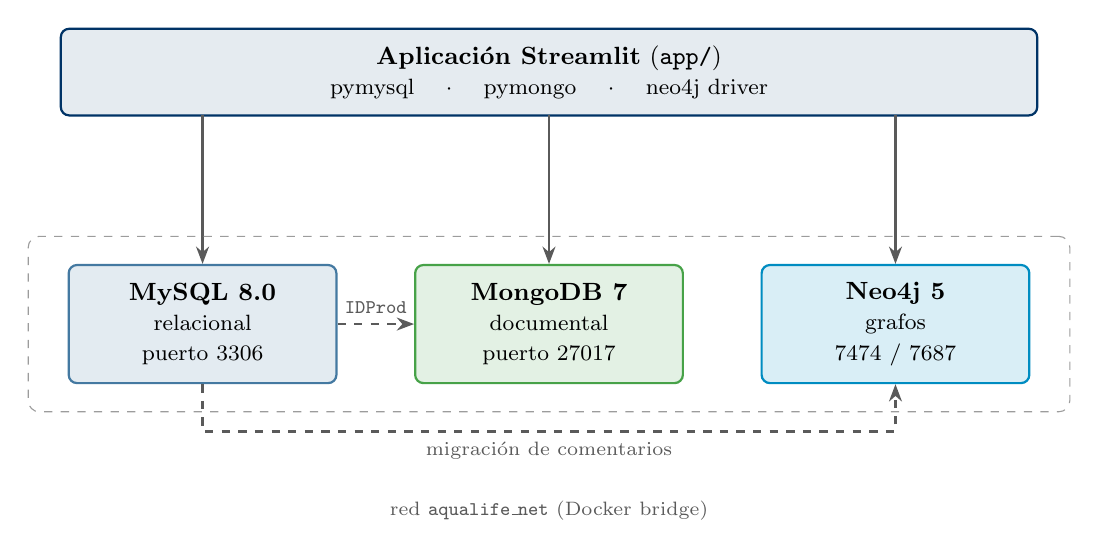
\begin{tikzpicture}[
    box/.style={draw, rounded corners=3pt, minimum height=1.5cm, minimum width=3.4cm, align=center, font=\small, thick},
    app/.style={box, fill=azulUH!10, draw=azulUH, minimum width=12.4cm, minimum height=1.1cm},
    arr/.style={-{Stealth[length=2.2mm]}, thick, color=grisUH}
]
\node[app] (st) at (0,0) {\textbf{Aplicación Streamlit} (\texttt{app/})\\ \footnotesize pymysql \quad $\cdot$ \quad pymongo \quad $\cdot$ \quad neo4j driver};
\node[box, fill=sqlcol!15, draw=sqlcol] (my) at (-4.4,-3.2) {\textbf{MySQL 8.0}\\ \footnotesize relacional\\ \footnotesize puerto 3306};
\node[box, fill=mongocol!15, draw=mongocol] (mo) at (0,-3.2) {\textbf{MongoDB 7}\\ \footnotesize documental\\ \footnotesize puerto 27017};
\node[box, fill=neocol!15, draw=neocol] (ne) at (4.4,-3.2) {\textbf{Neo4j 5}\\ \footnotesize grafos\\ \footnotesize 7474 / 7687};
\draw[arr] (-4.4,-0.55) -- (my.north);
\draw[arr] (0,-0.55) -- (mo.north);
\draw[arr] (4.4,-0.55) -- (ne.north);
\draw[arr, dashed] (my.east) -- node[above, font=\scriptsize, color=grisUH]{\texttt{IDProd}} (mo.west);
\draw[arr, dashed] (my.south) -- ++(0,-0.6) -| node[below, pos=0.25, font=\scriptsize, color=grisUH]{migración de comentarios} (ne.south);
\node[draw=grisUH!60, dashed, rounded corners=4pt, fit=(my)(mo)(ne), inner xsep=0.5cm, inner ysep=0.35cm] (red) {};
\node[font=\scriptsize, color=grisUH, anchor=north] at ([yshift=-1.0cm]red.south) {red \texttt{aqualife\_net} (Docker bridge)};
\end{tikzpicture}
\caption{Arquitectura del sistema. Las flechas discontinuas indican la vinculación de identificadores con MongoDB (\texttt{IDProd}) y la migración de datos hacia Neo4j.}
\label{fig:arq}
\end{figure}

\subsection{Modelo entidad-relación}
La Figura~\ref{fig:er} muestra el diagrama de entidades y atributos del modelo relacional principal.

\begin{figure}[H]
\centering
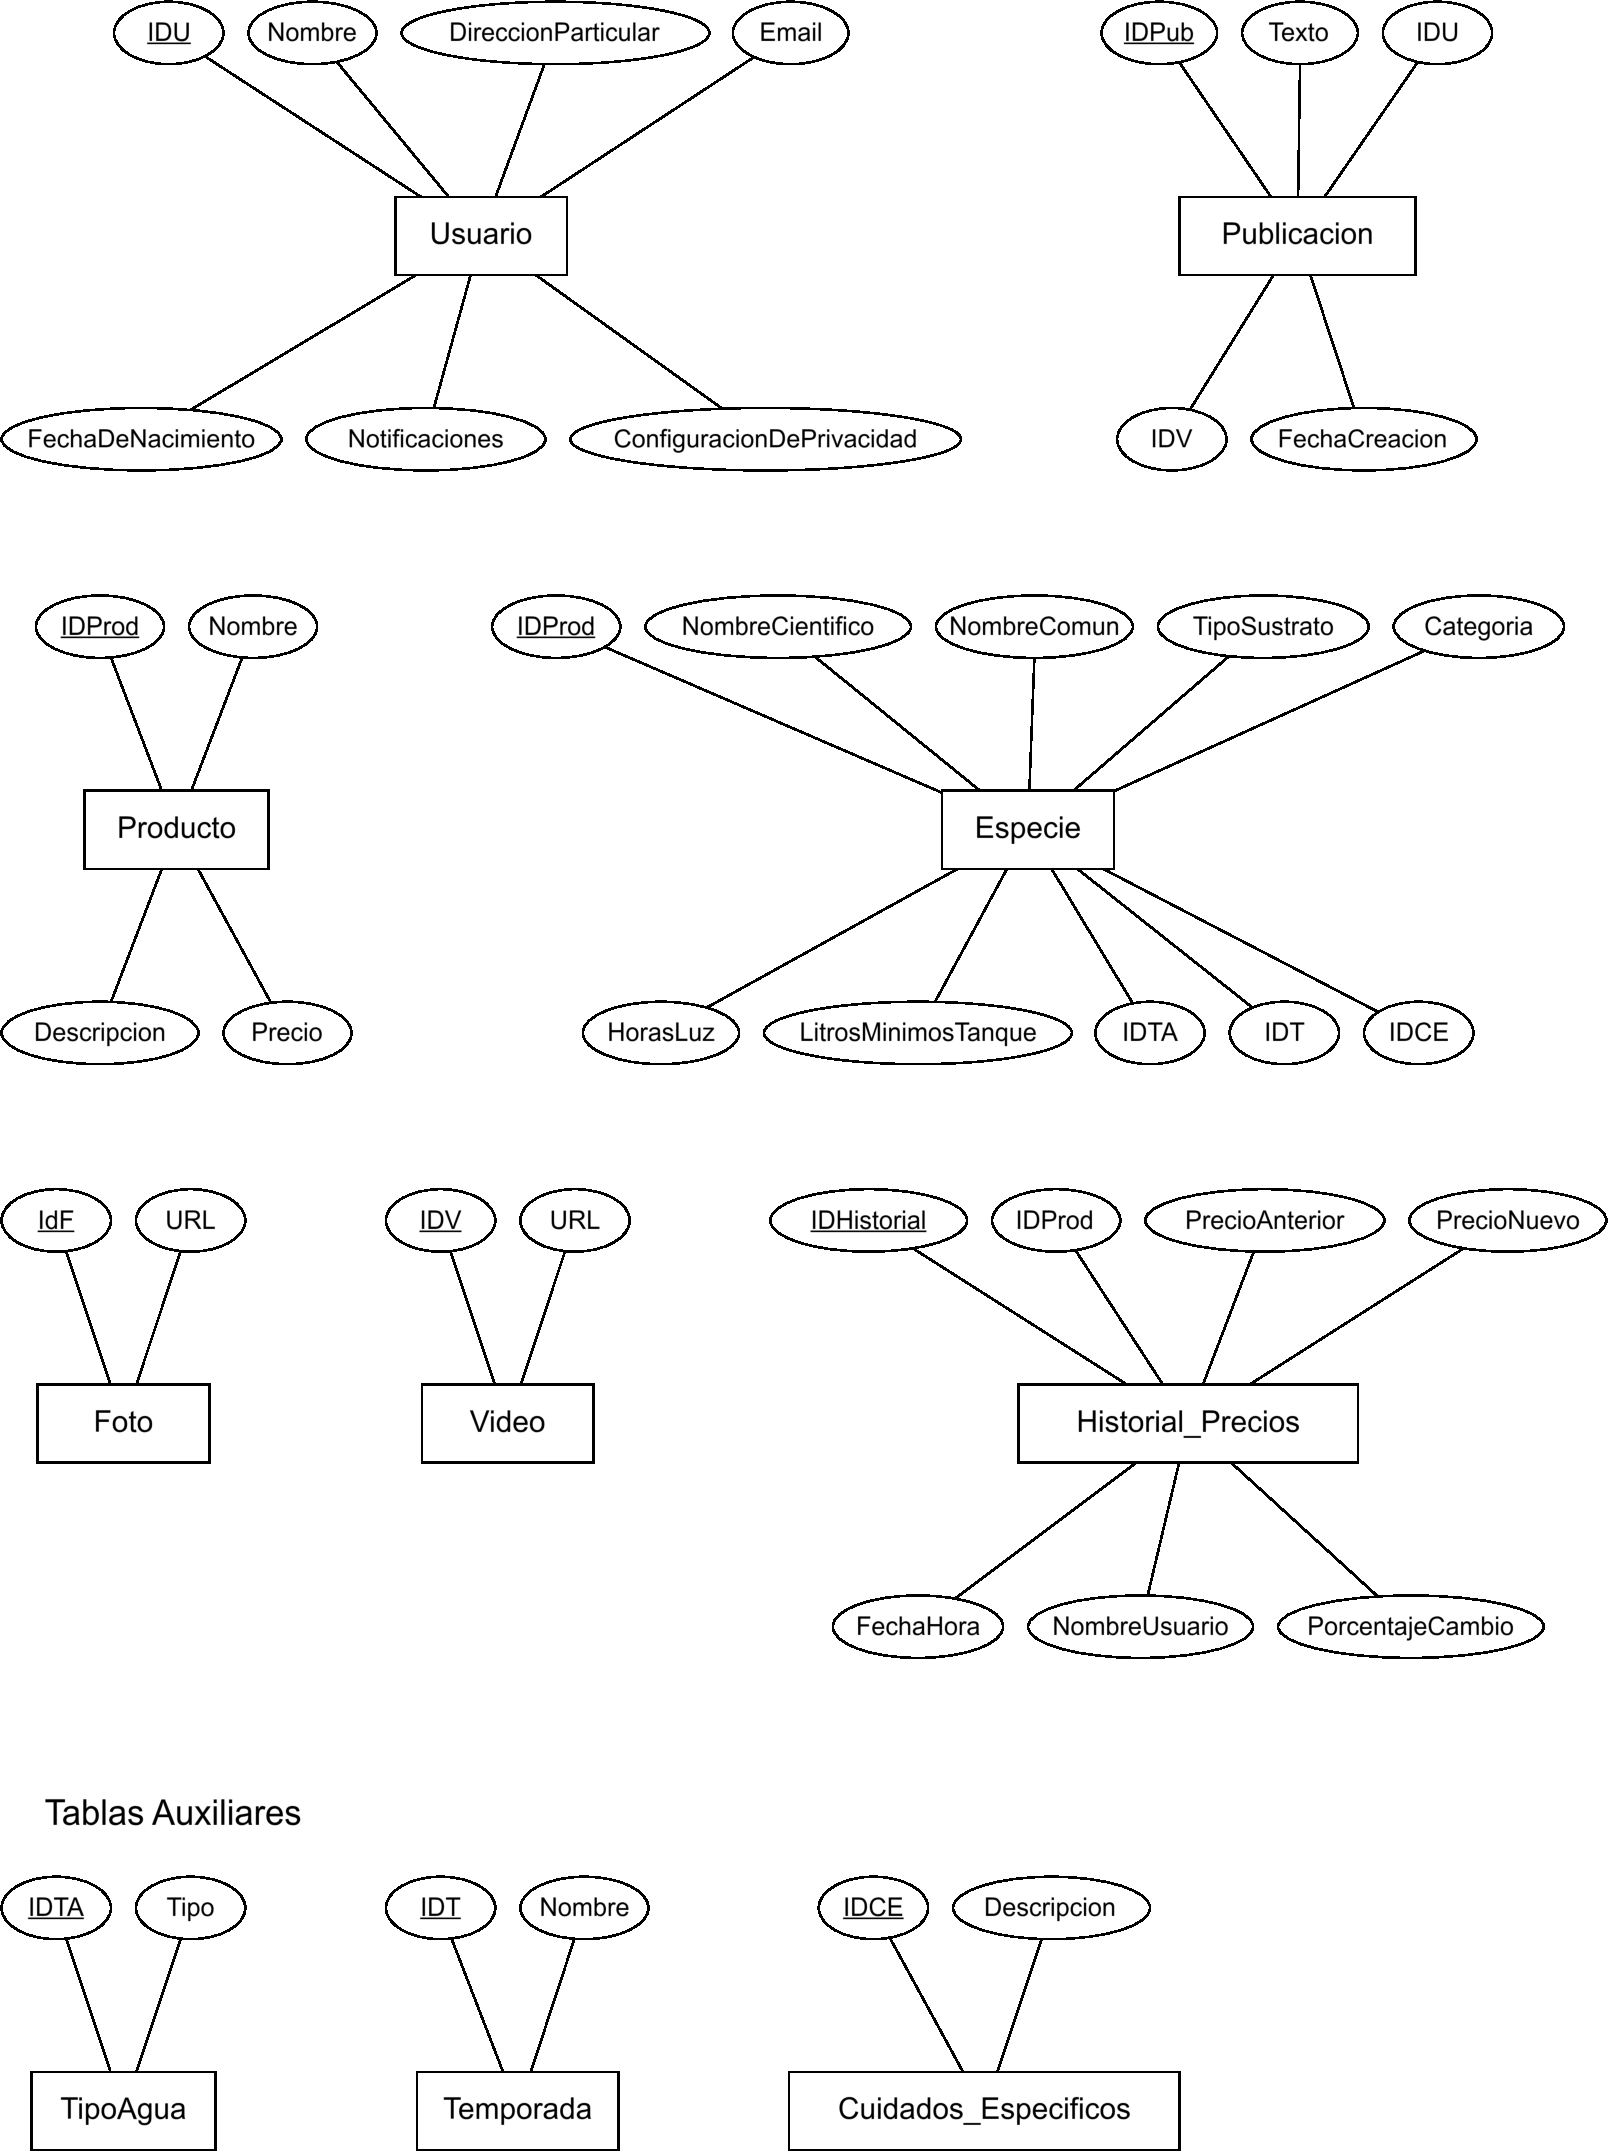
\includegraphics[width=\textwidth]{Entidades_y_atributos.pdf}
\caption{Diagrama de entidades y atributos (modelo relacional).}
\label{fig:er}
\end{figure}

\subsection{Diagrama de relaciones}
La Figura~\ref{fig:rel} muestra las relaciones entre las tablas principales.

\begin{figure}[H]
\centering
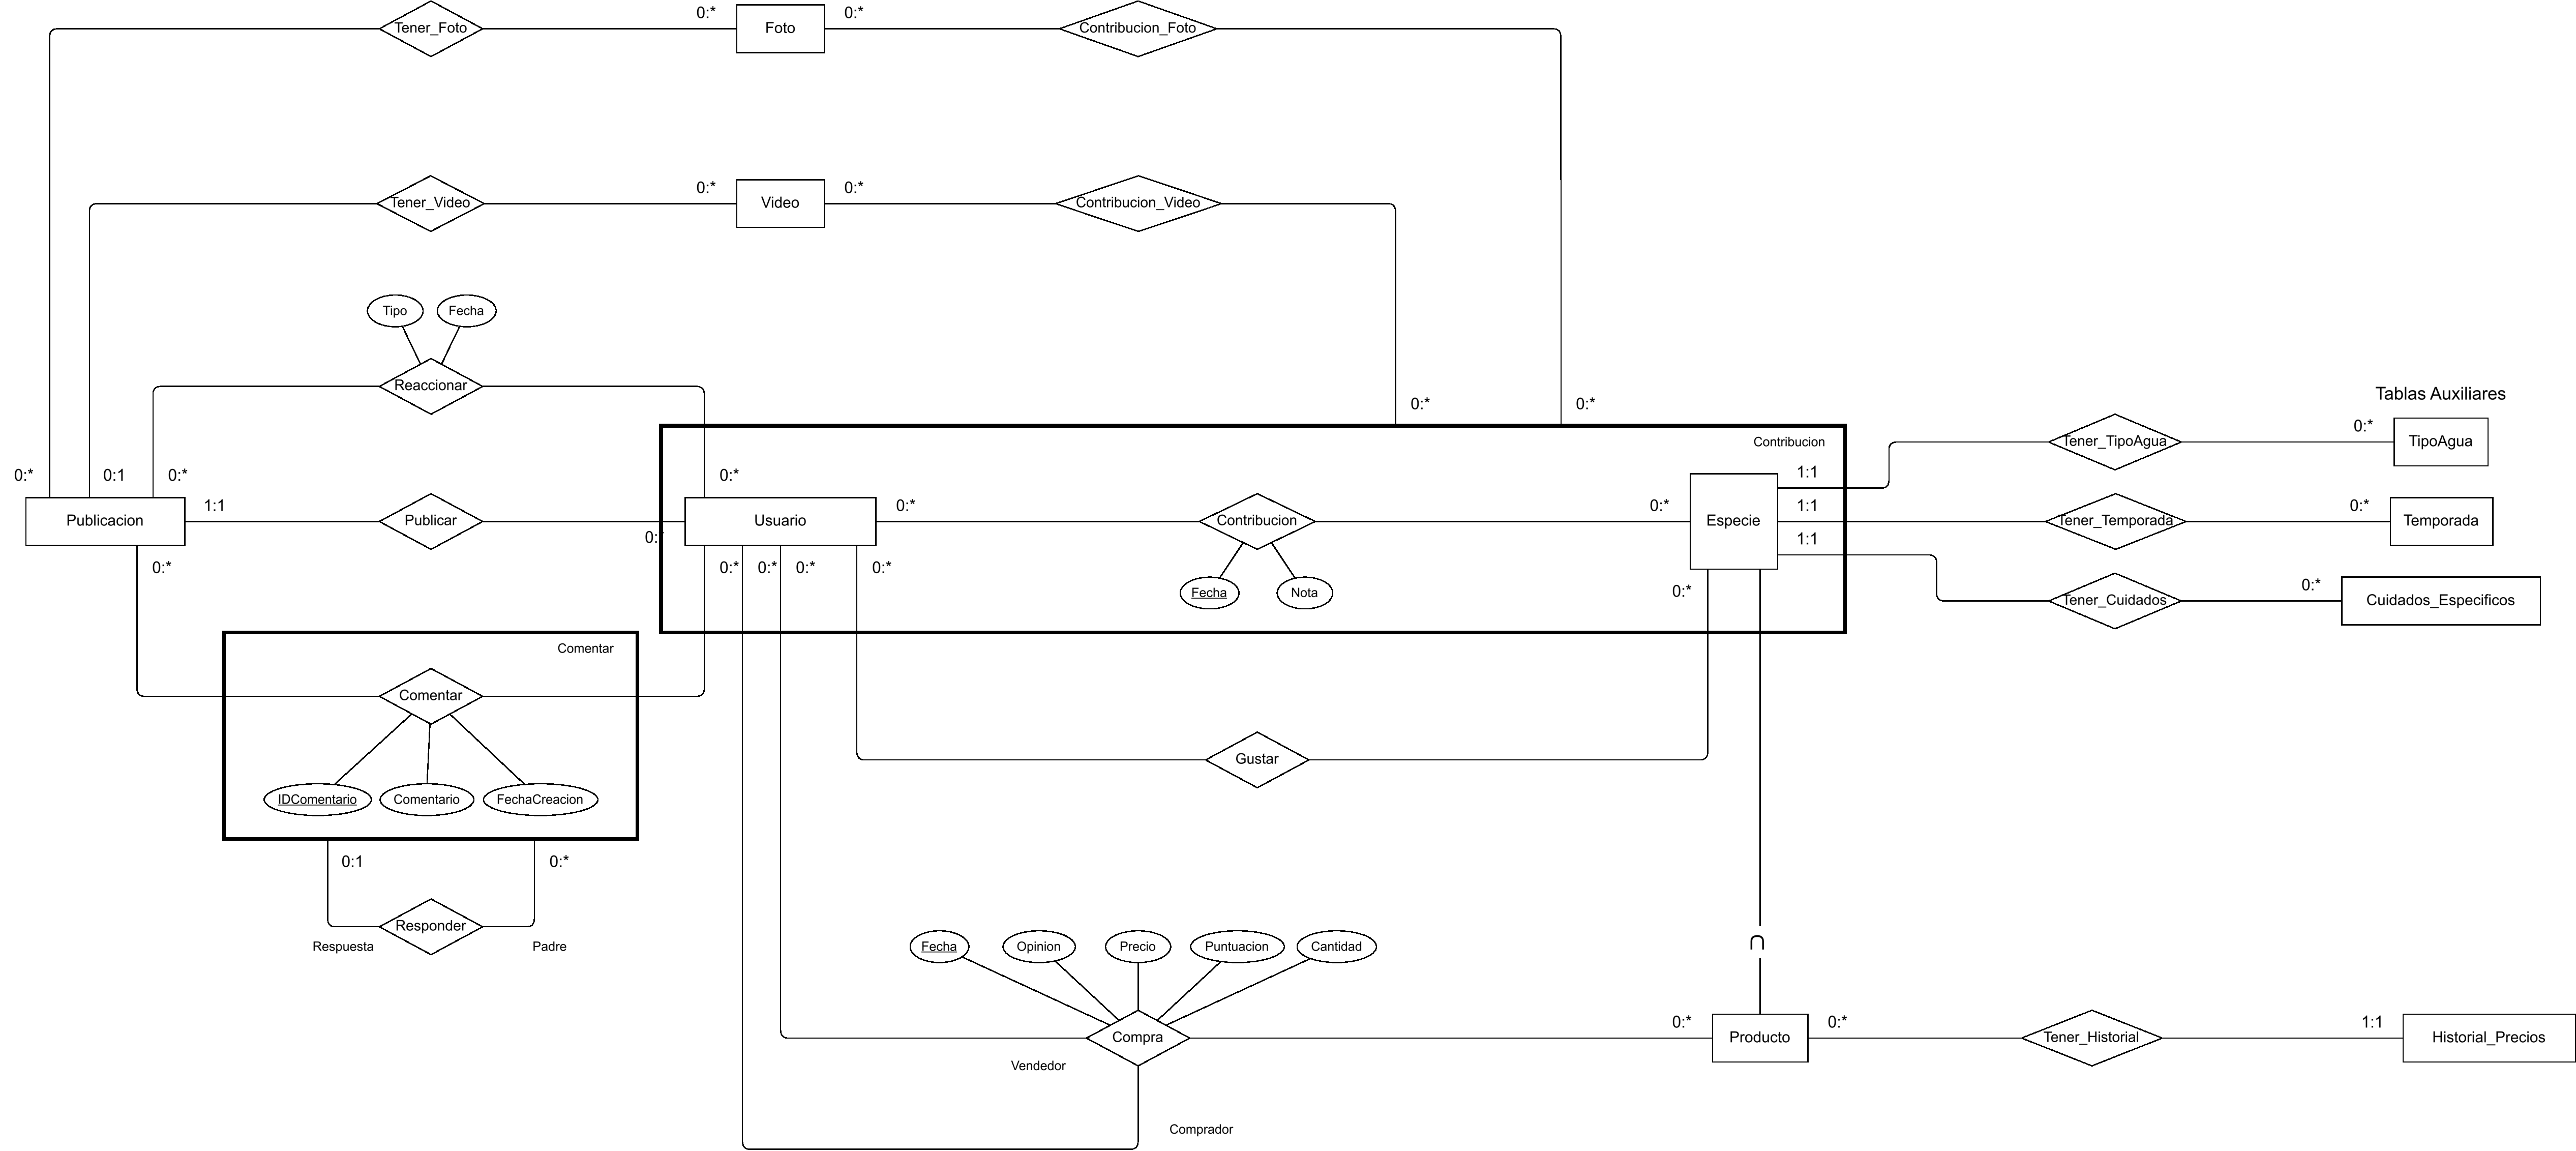
\includegraphics[width=\textwidth]{Relaciones.pdf}
\caption{Diagrama de relaciones entre tablas.}
\label{fig:rel}
\end{figure}

%=====================================================================
\section{Modelo relacional (MySQL)}\label{sec:rel}
%=====================================================================

\subsection{Papel del modelo relacional}
MySQL es el modelo principal del sistema. Contiene las entidades centrales y fuertemente estructuradas: usuarios, publicaciones, reacciones, compras, contribuciones, especies y productos. Para este tipo de datos, el modelo relacional es la opción natural: esquema fijo y conocido, integridad referencial mediante claves, transacciones ACID y un lenguaje de consulta (SQL) adecuado para agregaciones y combinaciones entre varias entidades, que son la base de las consultas analíticas del proyecto.

\subsection{Generación reproducible de los datos}
Los datos no se cargan a mano: un script Python (\texttt{generate\_init\_sql.py}) genera el archivo \texttt{init.sql} con datos aleatorios pero \textbf{deterministas}, fijando la semilla aleatoria \textbf{33} y una fecha de referencia \textbf{2026-01-01}. El volumen resultante ronda los 7 millones de filas, de las cuales aproximadamente 1,1 millones son comentarios. Las decisiones de diseño asociadas son las siguientes:

\begin{itemize}[leftmargin=1.5em]
    \item \textbf{Semilla fija y fecha de referencia:} garantizan que todos los integrantes, y el evaluador, trabajen con exactamente los mismos datos, de forma que los resultados de las consultas sean comparables y repetibles.
    \item \textbf{Verificación por hash SHA-256:} el script \texttt{000-hash-init.sh} comprueba la integridad de \texttt{init.sql} antes de cargarlo. El repositorio documenta el hash esperado y un comando para verificarlo, lo que detecta cualquier divergencia en la generación.
    \item \textbf{Orden de ejecución por nombre:} la imagen oficial de MySQL ejecuta los archivos de \texttt{docker-entrypoint-initdb.d} en orden alfabético. Los prefijos \texttt{000-} y \texttt{zzz-} aprovechan esto para que la verificación se ejecute la primera y la limpieza (\texttt{zzz-cleanup.sh}, que elimina \texttt{init.sql} tras la carga) la última.
    \item \textbf{Imagen con datos precargados:} el \texttt{Dockerfile} incorpora \texttt{init.sql} a la imagen, por lo que no depende de archivos externos en tiempo de ejecución.
\end{itemize}

\subsection{Ajustes de MySQL para la carga masiva}
Cargar unos 7 millones de filas con la configuración por defecto es lento. El servicio \texttt{mysqllab} arranca con parámetros orientados a la carga inicial, resumidos en la Tabla~\ref{tab:mysqlparams}.

\begin{table}[H]
\centering
\small
\begin{tabular}{
    >{\raggedright\arraybackslash}p{5.2cm}
    >{\raggedright\arraybackslash}p{9.0cm}}
\toprule
\textbf{Parámetro} & \textbf{Propósito} \\
\midrule
\texttt{max-allowed-packet=512M} & Permite sentencias \texttt{INSERT} de gran tamaño generadas por el script de datos. \\
\texttt{innodb-buffer-pool-size=512M} & Aumenta la caché de páginas e índices de InnoDB durante la carga. \\
\texttt{innodb-redo-log-\allowbreak capacity=512M} & Un registro de rehacer mayor reduce la frecuencia de \textit{checkpoints} forzados. \\
\texttt{innodb-flush-method=O\_DIRECT} & Evita la doble caché entre InnoDB y el sistema operativo. \\
\texttt{innodb-flush-log-\allowbreak at-trx-commit=2} & Vuelca el registro al sistema operativo en cada \textit{commit} y a disco cada segundo, en lugar de en cada transacción. \\
\texttt{sync-binlog=0} & No fuerza la sincronización a disco del registro binario. \\
\bottomrule
\end{tabular}
\caption{Parámetros de MySQL orientados a la carga masiva.}
\label{tab:mysqlparams}
\end{table}

\nota{Compromiso de durabilidad: los dos últimos parámetros relajan la garantía de durabilidad (ante una caída del sistema operativo podría perderse del orden de un segundo de transacciones). Es una decisión aceptable en un entorno académico con datos regenerables, pero no sería adecuada para un entorno de producción.}

\subsection{Consultas y objetos de base de datos}
Todas las consultas utilizan \textbf{SQL nativo, sin ORM}, de modo que la lógica queda explícita y evaluable. La Tabla~\ref{tab:consultas} lista los archivos de la carpeta \texttt{sql/}.

\begin{table}[H]
\centering
\small
\begin{tabular}{
    >{\raggedright\arraybackslash}p{3.1cm}
    >{\raggedright\arraybackslash}p{1.1cm}
    >{\raggedright\arraybackslash}p{9.6cm}}
\toprule
\textbf{Archivo} & \textbf{Tarea} & \textbf{Descripción} \\
\midrule
\texttt{3\_a.sql} & 3.a & Termómetro: reacciones totales por publicación, con datos del post y del autor. \\
\texttt{3\_b.sql} & 3.b & Publicaciones mejor recibidas: reacciones positivas frente a negativas. \\
\texttt{3\_c.sql} & 3.c & Perfil demográfico: distribución de edades en rangos de 10 años. \\
\texttt{3\_d.sql} & 3.d & Tendencias por tipo de agua a partir de las bitácoras de mantenimiento. \\
\texttt{3\_e.sql} & 3.e & Los 5 vendedores mejor calificados. \\
\texttt{3\_f.sql} & 3.f & \textit{Trigger} \texttt{tgr\_auditar\_precio} y tabla \texttt{Historial\_Precios}. \\
\texttt{3\_g.sql} & 3.g & Procedimiento \texttt{sp\_analisis\_usuario(id\_usuario, fecha\_inicio, fecha\_fin)}. \\
\texttt{3\_h.sql} & 3.h & Top 5 \textit{influencers}, especies más destacadas, \textit{lift} de ventas y tasa de conversión. \\
\texttt{3\_i.sql} & 3.i & Detección de patrones anómalos en vendedores mediante un Índice de Sospecha. \\
\texttt{comentarios.sql} & -- & Esquema de la tabla \texttt{Comentar} y procedimientos: \texttt{sp\_obtener\_hilo\_comentarios} (CTE recursivo para recuperar hilos completos) y \texttt{sp\_analisis\_usuario}. \\
\bottomrule
\end{tabular}
\caption{Consultas y objetos de base de datos del modelo relacional.}
\label{tab:consultas}
\end{table}

\subsection{Procedimiento almacenado \texttt{sp\_obtener\_hilo\_comentarios}}
Este procedimiento, definido en \texttt{comentarios.sql}, recupera el hilo completo de comentarios de una publicación mediante una expresión de tabla común recursiva (\texttt{WITH RECURSIVE}). El caso base selecciona los comentarios raíz (\texttt{IDPadre IS NULL}) de la publicación indicada, asignándoles nivel 0. La parte recursiva une cada comentario con sus respuestas mediante \texttt{IDPadre = IDComentario}, incrementando el nivel en cada iteración. El resultado incluye: \texttt{IDComentario}, \texttt{IDPadre}, \texttt{Comentario}, \texttt{Nombre} del autor, \texttt{FechaCreacion} y \texttt{Nivel} de profundidad. Una unión final con \texttt{Usuario} obtiene el nombre del autor. El procedimiento evita funciones de ventana y usa \texttt{UNION ALL} en la parte recursiva, conforme a los requisitos del enunciado.

\subsection{Justificación de los objetos programables}
\begin{itemize}[leftmargin=1.5em]
    \item \textbf{\textit{Trigger} de auditoría de precios (\texttt{tgr\_auditar\_precio}):} el historial de precios se registra dentro de la propia base de datos, en el momento en que cambia el precio de un producto. Así la auditoría no depende de que cada aplicación cliente se acuerde de registrarla, y no puede omitirse por error.
    \item \textbf{Procedimiento almacenado \texttt{sp\_analisis\_usuario}:} encapsula una consulta compleja y parametrizada (usuario y rango de fechas) en el servidor, lo que reduce el tráfico entre aplicación y base de datos y centraliza la lógica analítica en un único lugar reutilizable.
    \item \textbf{Índice de Sospecha (3.i):} resume en una única métrica varios indicadores de comportamiento anómalo de los vendedores, lo que facilita ordenar y priorizar los casos a revisar.
\end{itemize}

\subsection{Índices adicionales para optimización de consultas}
\label{sec:indices}
Para garantizar el rendimiento de las consultas analíticas (3.a--3.i) y el procedimiento \texttt{sp\_analisis\_usuario} sobre volúmenes de ~1,1M comentarios y ~7M filas totales, el script \texttt{generate\_init\_sql.py} crea los siguientes índices secundarios tras la carga masiva (prioridad $\ge$ 8/10):

\begin{table}[H]
\centering
\small
\begin{tabular}{
    >{\raggedright\arraybackslash}p{3.5cm}
    >{\raggedright\arraybackslash}p{10.3cm}}
\toprule
\textbf{Índice} & \textbf{Justificación} \\
\midrule
\texttt{Comentar(IDPub, IDPadre)} & CTE recursivo \texttt{sp\_obtener\_hilo\_comentarios}: caso base \texttt{WHERE IDPub=? AND IDPadre IS NULL} y JOIN recursivo \texttt{ON respuesta.IDPadre = hilo.IDComentario AND respuesta.IDPub = hilo.IDPub}. Sin compuesto, MySQL escanea todo \texttt{IDPub} y luego filtra \texttt{IDPadre}. \\
\midrule
\texttt{Compra(IDUV, IDProd, Fecha)} & Consultas 3.e (top vendedores) y 3.i (\texttt{variacion\_mensual}, \texttt{resumen\_calificaciones}): agrupación por vendedor + producto + fecha. \\
\texttt{Compra(IDUC, Fecha)} & SP \texttt{sp\_analisis\_usuario}: \texttt{total\_compras} + \texttt{monto\_gastado} por usuario en rango de fechas. \\
\texttt{Publicacion(IDU, FechaCreacion)} & SP: \texttt{total\_publicaciones} por usuario en rango de fechas. \\
\texttt{Reaccionar(IDU, Fecha)} & SP: \texttt{total\_reacciones\_dadas} por usuario en rango de fechas. \\
\texttt{Comentar(IDU, FechaCreacion)} & SP: \texttt{total\_comentarios} por usuario en rango de fechas. \\
\texttt{Contribucion(IDU, Fecha)} & SP: \texttt{total\_contribuciones} por usuario en rango de fechas. \\
\midrule
\texttt{Reaccionar(IDPub)} & Consultas 3.a, 3.b, 3.h: JOIN \texttt{Reaccionar.IDPub = Publicacion.IDPub}. FK no crea índice en tabla referenciada (MySQL 8). \\
\texttt{Contribucion(IDProd)} & Consultas 3.d, 3.h: JOIN \texttt{Contribucion.IDProd = Especie.IDProd}. \\
\texttt{Especie(IDTA)} & Consulta 3.d: JOIN \texttt{Especie.IDTA = TipoAgua.IDTA}. \\
\texttt{Compra(IDUV, Puntuacion)} & Consultas 3.i (\texttt{resumen\_calificaciones}), 3.e: agrupación y filtro por puntuaciones 1--5. \\
\bottomrule
\end{tabular}
\caption{Índices secundarios creados para optimizar consultas analíticas y SP. Definidos en \texttt{generate\_init\_sql.py}, sección \textit{ÍNDICES ADICIONALES}.}
\label{tab:indices}
\end{table}

Los índices se crean \textbf{tras la carga masiva} (no antes) para no penalizar la velocidad de inserción de los ~7M de filas. El script fija \texttt{innodb\_flush\_log\_at\_trx\_commit=1} y \texttt{sync\_binlog=1} en \texttt{docker-compose.yml} (configuración duradera de producción) antes de crearlos.

%=====================================================================
\section{Modelo documental (MongoDB): documentación jerárquica de especies}\label{sec:doc}
%=====================================================================

\subsection{Justificación del modelo documental}
La implementación del sistema de documentación jerárquica para las especies de AquaLife requiere una solución de almacenamiento que se adapte a la naturaleza de los datos. Se optó por una base de datos NoSQL orientada a documentos (MongoDB) debido al \textbf{polimorfismo y las estructuras variables} de los documentos secundarios. A diferencia del modelo relacional, donde incluir documentos como certificados sanitarios, análisis de agua o guías de alimentación obligaría a crear múltiples tablas con numerosos campos nulos (\texttt{NULL}), MongoDB permite que documentos con diferentes formatos y atributos coexistan de manera natural dentro de un mismo arreglo de subdocumentos.

Asimismo, el modelo documental ofrece una \textbf{jerarquía natural}. El formato JSON/BSON está diseñado para representar estructuras de árbol, lo que permite anidar la documentación secundaria directamente dentro de la ficha de la especie sin necesidad de costosas operaciones \texttt{JOIN}. Finalmente, para garantizar la \textbf{consistencia de los identificadores} y cumplir el requisito de que los atributos tengan el mismo nombre en SQL y NoSQL, el documento principal incluye un campo \texttt{IDProd} cuyo valor coincide exactamente con la clave primaria \texttt{IDProd} de la tabla \texttt{Especie} en MySQL. El identificador interno de MongoDB (\texttt{\_id}) es un \texttt{ObjectId} autogenerado, mientras que \texttt{IDProd} es el campo de negocio que permite la trazabilidad entre ambos sistemas.

\subsection{Elección del patrón: embebido frente a referencial}
Para modelar la relación uno a muchos (1:*) entre la ficha de especie y sus documentos secundarios, se evaluó el uso de referencias (documentos separados) frente al embebido (documentos anidados). La decisión se fundamentó en la \textbf{Regla de Oro de MongoDB}: \textit{``Data that is accessed together should be stored together''} (los datos a los que se accede juntos deben almacenarse juntos). Dado que el requerimiento exige consultar una especie y obtener inmediatamente todos sus documentos jerárquicamente, el patrón de \textbf{embebido (\textit{embedding})} es el más adecuado.

Esta decisión se respalda aplicando las siguientes directrices de diseño:
\begin{itemize}[leftmargin=1.5em]
    \item \textbf{Simplicidad y \textit{go together}:} agrupar los documentos simplifica el código de la aplicación y representa fielmente la relación ``tiene-un'' (una especie \textit{tiene} documentos).
    \item \textbf{Atomicidad de consulta:} la aplicación consulta la ficha completa de una vez, lo cual se resuelve con una sola operación de lectura sin usar \texttt{\$lookup}.
    \item \textbf{Cardinalidad e individualidad:} el número de documentos por especie es finito (no es un arreglo ilimitado) y un documento secundario no tiene sentido ni existencia por sí solo sin la especie a la que pertenece.
\end{itemize}

\subsection{Estructura conceptual del documento}
A modo ilustrativo, la ficha de una especie se organiza como un documento principal que contiene el campo \texttt{IDProd} (clave de negocio coincidente con MySQL) y un arreglo \texttt{DocumentosSecundarios} con documentos de tipos distintos, todos usando PascalCase para coincidir con los nombres de columna en SQL:

\begin{lstlisting}
{
  "IDProd": 87,
  "NombreComun": "Pez Cirujano",
  "NombreCientifico": "Acanthurus leucosternon",
  "Categoria": "Pez",
  "TipoSustrato": "Roca volcánica",
  "HorasLuz": 9,
  "LitrosMinimosTanque": 20,
  "IDTA": 8,
  "IDT": 2,
  "IDCE": 16,
  "Descripcion": "Pez: Pez Cirujano (Acanthurus leucosternon).",
  "DocumentosSecundarios": [
    { "Tipo": "Certificado Sanitario",
      "Fecha": "2024-03-15T00:00:00",
      "EstadoSalud": "Óptimo",
      "LibreParasitos": true,
      "VeterinarioResponsable": "Dr. Aqua" },
    { "Tipo": "Analisis de Agua",
      "FechaAnalisis": "2024-07-22T00:00:00",
      "Parametros": { "Ph": 7.8, "DurezaGh": 10, ... } },
    { "Tipo": "Guia de Alimentacion",
      "Temporada": "Verano",
      "DietaRecomendada": "Artemia",
      "FrecuenciaDiaria": "2 veces al día" }
  ]
}
\end{lstlisting}

Cada elemento del arreglo puede tener atributos distintos a los demás, sin necesidad de columnas nulas ni de tablas adicionales. La aplicación consume esta colección desde el módulo \texttt{doc\_explorer.py}, que permite explorar los documentos jerárquicos de cada especie. Los 4000 documentos se generan con el script \texttt{scripts/ficha\_de\_especie\_mongodb.py}, que lee los datos de \texttt{Especie} y \texttt{Producto} en MySQL y los inserta en la colección \texttt{fichas\_especie} de la base de datos \texttt{AquaLifeDoc}.

\subsection{Cuándo no sería adecuado el embebido}
El patrón embebido tiene límites que conviene dejar explícitos. Si el número de documentos secundarios por especie creciera sin control, el documento podría acercarse al límite de 16~MB que impone MongoDB, y habría que pasar a referencias. Del mismo modo, si los documentos secundarios debieran consultarse o actualizarse de forma independiente y muy frecuente, o compartirse entre varias especies, el modelo referencial sería preferible. Las condiciones de AquaLife (conjunto finito, acceso conjunto y ausencia de existencia independiente) son las que hacen del embebido la mejor opción.

%=====================================================================
\section{Modelo de grafos (Neo4j): conversaciones en comentarios}\label{sec:grafos}
%=====================================================================

\subsection{Planteamiento del problema}
La implementación de conversaciones mediante comentarios requiere representar relaciones jerárquicas entre publicaciones y respuestas. Cada comentario puede constituir una entrada independiente o responder a otro comentario, dando lugar a estructuras recursivas conocidas como hilos de conversación. Para abordar este problema se desarrollaron dos implementaciones: una basada en el modelo relacional (MySQL) y otra mediante una base de datos orientada a grafos (Neo4j). Aunque ambas permiten representar y recuperar conversaciones con múltiples niveles de profundidad, difieren en la forma de modelar las relaciones y en los mecanismos empleados para recorrerlas.

\subsection{Diseño e implementación del modelo relacional}
En la implementación relacional, los comentarios se almacenan en la tabla \texttt{Comentar}. Cada registro contiene un identificador propio (\texttt{IDComentario}), el identificador del usuario que lo escribió (\texttt{IDU}), la publicación a la que pertenece (\texttt{IDPub}) y el contenido del comentario.

La característica fundamental de este diseño es el atributo \texttt{IDPadre}, que establece una relación autorreferenciada dentro de la propia tabla \texttt{Comentar}. Cuando un comentario constituye una entrada principal del hilo, este atributo toma el valor \texttt{NULL}. En cambio, cuando representa una respuesta, almacena el identificador del comentario al que responde.

\begin{itemize}[leftmargin=1.5em]
    \item Los comentarios principales tienen \texttt{IDPadre = NULL}.
    \item Las respuestas almacenan en \texttt{IDPadre} el identificador de su comentario padre.
    \item Las respuestas pueden convertirse, a su vez, en padres de nuevos comentarios.
\end{itemize}

Esta representación permite construir conversaciones de profundidad arbitraria sin necesidad de crear una tabla diferente para cada nivel de respuesta.

\subsubsection{Inserción de comentarios}
La función \texttt{add\_comment()} implementa la inserción de nuevos comentarios desde Python. Primero identifica al usuario mediante su nombre y, si no existe, lo incorpora a la tabla \texttt{Usuario}. Cuando se trata de una respuesta, se comprueba que el comentario padre exista y pertenezca a la misma publicación. Posteriormente, se inserta el nuevo comentario con su correspondiente referencia \texttt{IDPadre}. Las operaciones se ejecutan dentro de una transacción: si ocurre algún error, se realiza un \texttt{ROLLBACK}; en caso contrario, se confirma mediante \texttt{COMMIT}. Esto permite mantener la consistencia de las operaciones de inserción.

\subsubsection{Recuperación recursiva de un hilo}
La recuperación de una conversación completa se realiza mediante el procedimiento almacenado \texttt{sp\_obtener\_hilo\_comentarios}, implementado utilizando una expresión de tabla común recursiva (\texttt{WITH RECURSIVE}). El procedimiento comienza identificando los comentarios principales de una publicación, es decir, aquellos cuyo atributo \texttt{IDPadre} es \texttt{NULL}. Estos constituyen el caso base de la recursión y reciben un nivel inicial igual a cero. La parte recursiva incorpora las respuestas cuyo \texttt{IDPadre} coincide con el identificador de alguno de los comentarios previamente recuperados, incrementando el nivel en cada iteración, hasta que no existen nuevas respuestas que incorporar.

Además, el procedimiento realiza una unión con la tabla \texttt{Usuario} para recuperar el nombre del autor y devuelve: identificador del comentario, identificador del comentario padre, contenido, nombre del autor, fecha de creación y nivel de profundidad. La inclusión del atributo \texttt{Nivel} facilita la posterior representación jerárquica de la conversación en la aplicación.

\subsection{Diseño e implementación del modelo de grafos}
En la implementación con Neo4j, la conversación se representa mediante un grafo compuesto por nodos y relaciones. A diferencia del modelo relacional, donde la jerarquía se expresa mediante referencias entre registros, aquí las conexiones entre comentarios se representan explícitamente mediante aristas. Se utilizan tres tipos de nodos: \texttt{Usuario}, \texttt{Publicacion} y \texttt{Comentar}. Las relaciones principales son:

\begin{itemize}[leftmargin=1.5em]
    \item \texttt{ESCRIBIO}: conecta un usuario con el comentario que escribió.
    \item \texttt{EN\_PUBLICACION}: conecta un comentario con la publicación a la que pertenece.
    \item \texttt{RESPONDE\_A}: conecta un comentario con el comentario al que responde.
\end{itemize}

La relación \texttt{RESPONDE\_A} constituye el elemento central del diseño, puesto que permite representar directamente la estructura jerárquica de las conversaciones. Un comentario principal no necesita establecer una relación con otro comentario, mientras que cada respuesta incorpora una conexión hacia su comentario padre.

\subsubsection{Inserción de comentarios}
La función \texttt{add\_comment()} (en \texttt{app/neo4j\_db.py}) utiliza operaciones \texttt{MERGE} para crear o localizar los nodos correspondientes a usuarios, publicaciones y comentarios. Posteriormente, establece las relaciones que representan la autoría y la pertenencia a una publicación. Cuando el comentario es una respuesta, se verifica previamente la existencia del comentario padre \textbf{y que este pertenezca a la misma publicación} mediante un patrón \texttt{MATCH (parent:Comentar \{IDComentario: \$parent\})-[:EN\_PUBLICACION]->(p:Publicacion \{IDPub: \$pid\})}. Esto iguala la garantía de integridad del modelo relacional. Asimismo, se establecen restricciones de unicidad sobre los identificadores de usuarios, publicaciones y comentarios, evitando que existan múltiples nodos con el mismo identificador dentro de cada etiqueta.

\subsubsection{Recuperación de un hilo mediante recorridos del grafo}
La función \texttt{get\_thread()} utiliza el lenguaje Cypher para recuperar los comentarios pertenecientes a una publicación y sus relaciones jerárquicas. La consulta emplea un recorrido de longitud variable desde la raíz hacia abajo, devuelve el nivel de profundidad mediante \texttt{length(path)} y agrupa todos los resultados en una sola fila con \texttt{collect()} para evitar el cuello de botella de decodificación de miles de registros en el driver de Python:

\begin{lstlisting}
MATCH (p:Publicacion {IDPub: $pid})
    <-[:EN_PUBLICACION]-(root:Comentar)
WHERE NOT (root)-[:RESPONDE_A]->()

MATCH path = (root)<-[:RESPONDE_A*0..]-(c:Comentar)
OPTIONAL MATCH (c)<-[:ESCRIBIO]-(u:Usuario)

WITH c, u, length(path) AS level
ORDER BY c.IDComentario
RETURN collect({
    id: c.IDComentario,
    parent_id: c.IDPadre,
    text: c.Comentario,
    author: u.Nombre,
    created: toString(c.FechaCreacion),
    level: level
}) AS rows
\end{lstlisting}

El operador \texttt{*0..} permite recorrer cero o más relaciones de tipo \texttt{RESPONDE\_A} en dirección inversa (de padre a hijo), visitando cada nodo una sola vez. El campo \texttt{IDPadre} almacenado en el nodo evita un \texttt{MATCH} adicional para obtener el padre. La fecha se devuelve como cadena con \texttt{toString()} para evitar la conversión costosa de objetos \texttt{datetime} en el driver. El resultado es una lista de mapas con la misma estructura que el procedimiento SQL: \texttt{id}, \texttt{parent\_id}, \texttt{text}, \texttt{author}, \texttt{created}, \texttt{level}.

\subsection{Comparación de ambos diseños}

\subsubsection{Representación de las relaciones}
En el modelo relacional, las relaciones jerárquicas se almacenan como valores dentro de una columna: el atributo \texttt{IDPadre} establece una referencia entre dos registros de la misma tabla. Por tanto, la estructura de la conversación no se encuentra representada directamente, sino que debe reconstruirse mediante consultas que relacionen repetidamente los registros. En Neo4j, por el contrario, la jerarquía forma parte de la propia estructura del grafo: cada respuesta mantiene una relación explícita con su comentario padre, por lo que las conexiones pueden recorrerse directamente. Esta diferencia resulta especialmente relevante cuando se trabajan con conversaciones con múltiples niveles de anidamiento.

\subsubsection{Complejidad de las consultas}
En MySQL, la recuperación de un hilo completo requiere una consulta recursiva: el procedimiento debe definir un caso base, establecer la condición recursiva y controlar la incorporación de nuevos registros. Aunque los CTE recursivos resuelven el problema de manera elegante y sin establecer un límite fijo de profundidad, la consulta requiere una lógica adicional para reconstruir la jerarquía. En Neo4j, la misma operación se expresa mediante patrones de recorrido sobre las relaciones del grafo; las relaciones de longitud variable permiten recuperar los comentarios conectados sin implementar explícitamente una recursión mediante uniones sucesivas. Por consiguiente, Cypher ofrece una representación más natural e intuitiva de este tipo de consultas, especialmente cuando las relaciones entre los datos constituyen el elemento principal del problema.

\subsubsection{Integridad y consistencia de los datos}
El modelo relacional ofrece mecanismos consolidados para garantizar la integridad mediante restricciones, claves y transacciones. En la implementación desarrollada destaca la comprobación de que el comentario padre pertenezca a la misma publicación que la nueva respuesta, lo que evita establecer relaciones jerárquicas entre comentarios de conversaciones diferentes.

Neo4j también permite establecer restricciones de unicidad y utilizar transacciones. En la implementación actual, \texttt{add\_comment()} verifica que el comentario padre exista \textbf{y que pertenezca a la misma publicación} mediante el patrón \texttt{MATCH (parent)-[:EN\_PUBLICACION]->(p:Publicacion \{IDPub: \$pid\})}, igualando la garantía del modelo relacional.

\subsubsection{Mantenimiento y evolución del sistema}
El modelo relacional presenta la ventaja de utilizar una estructura conocida, organizada y ampliamente estandarizada. Su integración con aplicaciones Python y otros sistemas de información resulta directa, y permite aprovechar las herramientas habituales de administración y consulta de bases de datos SQL. Sin embargo, cuando las consultas dependen frecuentemente de relaciones recursivas, puede aumentar la complejidad de los procedimientos almacenados necesarios para recuperar la información.

En Neo4j, la representación explícita de las relaciones facilita la comprensión y modificación de la estructura de las conversaciones; por ejemplo, incorporar nuevas relaciones entre usuarios, comentarios y publicaciones puede resultar más natural. No obstante, requiere familiarizarse con Cypher y con las herramientas propias de las bases de datos orientadas a grafos, lo que puede representar una dificultad adicional en sistemas cuya infraestructura está diseñada principalmente alrededor de tecnologías relacionales.

\subsection{Resumen comparativo}
\begin{table}[H]
\centering
\small
\begin{tabular}{
    |>{\raggedright\arraybackslash}p{2.8cm}
    |>{\raggedright\arraybackslash}p{5.3cm}
    |>{\raggedright\arraybackslash}p{5.3cm}|
}
\hline
\textbf{Criterio} & \textbf{Modelo relacional (MySQL)} & \textbf{Modelo de grafos (Neo4j)} \\
\hline
Representación & Relación autorreferenciada mediante \texttt{IDPadre}. & Relaciones explícitas \texttt{RESPONDE\_A} entre nodos. \\
\hline
Estructura & Registros organizados en tablas. & Nodos y aristas que representan entidades y relaciones. \\
\hline
Recuperación del hilo & CTE recursivo mediante \texttt{WITH RECURSIVE}. & Recorrido de relaciones mediante patrones de longitud variable. \\
\hline
Profundidad & Se calcula explícitamente mediante el atributo \texttt{Nivel}. & Se devuelve explícitamente mediante \texttt{length(path)} en la consulta. \\
\hline
Integridad & Permite validar que padre e hijo pertenezcan a la misma publicación. & La implementación actual valida existencia del padre y su pertenencia a la publicación. \\
\hline
Mantenimiento & Estructura conocida y herramientas SQL ampliamente utilizadas. & Mayor flexibilidad para incorporar nuevas relaciones entre entidades. \\
\hline
Consultas relacionales & Adecuado para consultas estructuradas y operaciones sobre múltiples tablas. & No es su mecanismo principal de consulta. \\
\hline
Consultas de grafos & Requiere reconstruir las relaciones mediante consultas recursivas. & Permite expresar recorridos jerárquicos directamente. \\
\hline
\end{tabular}
\caption{Comparación de las implementaciones relacional y orientada a grafos.}
\label{tab:comparacion-modelos}
\end{table}

\subsection{Conclusiones sobre el modelo de conversaciones}
Ambos modelos permiten implementar correctamente un sistema de conversaciones con múltiples niveles de respuestas; la elección depende de las características del problema y de las operaciones más frecuentes. El modelo relacional es adecuado cuando el sistema requiere mantener información estructurada, realizar consultas sobre múltiples entidades y garantizar la consistencia mediante restricciones y transacciones; el CTE recursivo demuestra que SQL puede gestionar eficientemente estructuras jerárquicas sin recurrir a otra tecnología.

Por otra parte, el modelo orientado a grafos presenta una ventaja conceptual importante para este escenario: las conversaciones son, esencialmente, estructuras formadas por entidades conectadas mediante relaciones. Considerando la naturaleza del problema, se considera que \textbf{Neo4j resulta el modelo más apropiado para representar las conversaciones mediante comentarios}, puesto que la estructura jerárquica y las relaciones entre los elementos constituyen el aspecto central del sistema.

No obstante, esta elección no implica que MySQL sea incapaz de resolver el problema ni que Neo4j garantice por sí solo un mejor rendimiento. La implementación relacional ofrece una solución perfectamente válida y presenta ventajas importantes en cuanto a integridad y gestión transaccional. Para un sistema cuyo componente principal sea la navegación y exploración de conversaciones complejas, Neo4j ofrece una mayor correspondencia entre la naturaleza de los datos y su representación; si, por el contrario, los comentarios son solo una funcionalidad adicional dentro de una aplicación predominantemente relacional, MySQL puede ser más conveniente desde el punto de vista de la integración y la administración.

%=====================================================================
\section{Comparación global de los tres paradigmas}\label{sec:comp}
%=====================================================================

\begin{table}[H]
\centering
\small
\begin{tabular}{
    >{\raggedright\arraybackslash}p{2.4cm}
    >{\raggedright\arraybackslash}p{3.8cm}
    >{\raggedright\arraybackslash}p{3.8cm}
    >{\raggedright\arraybackslash}p{3.8cm}}
\toprule
\textbf{Aspecto} & \textbf{MySQL} & \textbf{MongoDB} & \textbf{Neo4j} \\
\midrule
Modelo de datos & Tablas y filas con esquema fijo. & Documentos JSON/BSON con esquema flexible. & Nodos y relaciones con propiedades. \\
Dato típico en AquaLife & Compras, reacciones, precios, usuarios. & Ficha de especie con documentos secundarios heterogéneos. & Hilos de comentarios anidados. \\
Fortaleza principal & Integridad, transacciones ACID y agregaciones. & Polimorfismo y jerarquías anidadas sin \texttt{JOIN}. & Recorridos de relaciones de profundidad variable. \\
Lenguaje de consulta & SQL. & API de consultas de MongoDB (\texttt{find}, agregaciones). & Cypher. \\
Punto débil en este contexto & Jerarquías recursivas requieren CTE. & Poca garantía de integridad entre documentos. & Requiere aprender Cypher y su infraestructura. \\
Criterio de elección & Datos estructurados y analítica. & Los datos se acceden y evolucionan juntos. & Las relaciones son el centro del problema. \\
\bottomrule
\end{tabular}
\caption{Comparación global de los tres paradigmas en el contexto de AquaLife.}
\end{table}

El criterio común que guía la distribución es adecuar el modelo a la \textbf{forma natural del dato}: tabular y relacional para las entidades de negocio, árbol de documentos para fichas heterogéneas y grafo para conversaciones. Ninguno de los tres paradigmas es superior en términos absolutos; la persistencia políglota permite usar cada uno donde aporta más, a costa de una mayor complejidad operativa (tres servicios que mantener) y de la necesidad de mantener coherentes los identificadores entre sistemas, como ocurre con \texttt{IDProd} entre MySQL y MongoDB.

%=====================================================================
\section{Conclusiones}\label{sec:concl}
%=====================================================================

AquaLife demuestra que un mismo dominio puede beneficiarse de varios modelos de datos cuando cada uno se asigna a la parte del problema que mejor representa. MySQL aporta integridad, transacciones y capacidad analítica para las entidades de negocio; MongoDB resuelve de forma natural la documentación heterogénea y jerárquica de las especies mediante documentos embebidos, usando nombres de campo idénticos a los de SQL (\texttt{IDProd}, \texttt{NombreComun}, \texttt{NombreCientifico}, \texttt{Categoria}, \texttt{TipoSustrato}, \texttt{HorasLuz}, \texttt{LitrosMinimosTanque}, \texttt{IDTA}, \texttt{IDT}, \texttt{IDCE}, \texttt{Descripcion}); y Neo4j representa de manera directa las conversaciones como un grafo de respuestas, con validación de integridad equivalente a la relacional y una consulta optimizada que devuelve el hilo completo con nivel de profundidad en una sola fila. El despliegue con Docker Compose, la generación determinista de datos (semilla 33, fecha de referencia 2026-01-01) y la verificación por hash hacen que el proyecto sea reproducible.

Como líneas de mejora futura, se sugiere: fijar versiones de imágenes en \texttt{docker-compose.yml} (ya aplicado: \texttt{mongo:7}, \texttt{neo4j:5}); externalizar credenciales mediante variables de entorno; revertir los ajustes de durabilidad de MySQL (\texttt{innodb-flush-log-at-trx-commit=2}, \texttt{sync-binlog=0}) tras la carga inicial; añadir validación \texttt{\$jsonSchema} en MongoDB; documentar planes de ejecución (\texttt{EXPLAIN} / \texttt{PROFILE}) para comparar rendimiento con índices adecuados (p.ej., \texttt{Comentar(IDPub, IDPadre)}); y mantener la medición separada de tiempo de servidor y cliente en Neo4j para evitar cuellos de botella en el driver.

\end{document}